\chapter{Aspectos Estad\'isticos de la Homolog\'ia Persistente}\label{chap:Cap5}cap 5

Por s\'i sola, la homolog\'ia persistente no toma en cuenta la naturaleza estoc\'astica de los datos
y la variabilidad intrinseca de las cantidades topol\'ogicas que infieren.
Buscamos ahora un acercamiento esta\'distico a la homolog\'ia persistente,
considerando que los datos son generados de alguna distribuci\'on desconocida.
Comenzamos dando varos resultados de consistencia para la inferencia de la homolog\'ia persistente.

\section{Resultados de Consistencia para la Homolog\'ia Persistente}

Sup\'ongase que observamos $n$ puntos $\cpar{X_{1},\dots,X_{n}}$ en un espacio m\'etrico
$\cpar{M,\rho}$ obtenidas i. i. d. de una medida de probabilidad desconocida $\mu$ con
soporte compacto $\mathbb{X}_{\mu}$ la distancia de Gromov-Hausdorff nos permite comparar
$\mathbb{X}_{\mu}$ con otros espacios m\'etricos compactos no necesariamente encajados en $M$.
Definimos a continuaci\'on, $\hat{\mathbb{X}}$ un estimador de $\mathbb{X}_{\mu}$
como una funci\'on de $X_{1},\dots,X_{n}$ que toma valores en el conjunto de espacios m\'etricos compactos.

Sean $\mathrm{Filt}\cpar{\mathbb{X}_{\mu}}$ y $\mathrm{Filt}\cpar{\hat{\mathbb{X}}}$
dos filtraciones definidas en $\mathbb{X}_{\mu}$ y $\hat{\mathbb{X}}$.
Con el teorema \ref{teo:4.9} hemos visto que una estrategia natural
para estimar la homologi\'ia persistente de $\mathrm{Filt}\cpar{\mathbb{X}_{\mu}}$
consiste en estimar el soporte de $\hat{\mathbb{X}}$.
N\'otese que en algunos casos, el espacio $M$ puede ser desconocido
y las observaciones $X_{1},\dots,X_{n}$ solo se conocen mediante de sus distancias por pares
$\rho\cpar{X_{i}, X_{j}}$, $i$, $j = 1,\dots,n$.
La distancia de Gromov-Hausforff nos permite considerar el conjunto de observaciones
como un espacio m\'etrico abstracto de cardinalidad $n$,
independietemente de la manera en la que esta encajado en $M$.
Esta estructura general incluye el acercamiento m\'as est\'andar
que consiste en estamar el soporte con respecto a la distancia de Hausdorff
restringiendo los valores de $\hat{\mathbb{X}}$ a los conjuntos compactos en $M$.

El conjunto finito $\mathbb{X}_{n}:=\cllav{X_{1},\dots,X_{2}}$
es un estimador natural para el soporte de $\mathbb{X}_{\mu}$.
En muchos de los contextos que veremos a continuaci\'on,
$\mathbb{X}_{\mu}$ muestra tasas de convergencia \'optimas
con respecto a la ditancia de Hausdorff.
Para algunas constantes $a,b>0$, decimos que $\mu$ satisface el supuesto
$\cpar{a,b}$-est\'andar si para cualquier $x\in\mathbb{X}_{\mu}$ y cualquer $r>0$,
\begin{equation}
    \mu\cpar{B\cpar{x,r}}\geq\min\cpar{ar^{b},1}.
\end{equation}

Este supuesto es ampliamente usado en la literatura de la estimaci\'on de conjuntos
bajo la distancia de Hausdorff
(Cuevas y Rodriguez-Casal, 2004\cite{CuevasRodriguezCasal2004};
Singh et al., 2009\cite{Singh2009}).
Bajo este supuesto, puede deducirse que la tasa de convergencia de
$\mathrm{dgm}\cpar{\mathrm{Filt}\cpar{\mathbb{X}_{n}}}$ a
$\mathrm{dgm}\cpar{\mathrm{Filt}\cpar{\mathbb{X}_{\mu}}}$
para la m\'etrica de cuello de botella es acotada superiormente por
$O\cpar{\frac{\log n}{n}}^{1/b}$. M\'as precisamente, esta tasa
acota superiormente la tasa de convergencia minimax sobre el conjunta de medidas
de probabilidad en el espacio m\'etrico $\cpar{M, \rho}$ satisfaciendo el supuesto
$\cpar{a,b}$-est\'andar en $M$.

\begin{teorema}
    Chazal et al. (2014)\cite{Chazal2014b} para algunas constantes positivas, $a$ y $b$, sea
    \begin{equation*}
        \mathcal{P}:=\cllav{\mu \text{ en } M |
        \mathbb{X}_{\mu}\text{ es compacto y }\forall x\in\mathbb{X}_{\mu},\forall r>0,\hspace{4pt}
        \mu\cpar{B\cpar{x,r}}\geq\min\cpar{1,ar^{b}}}
    \end{equation*}
    Entonces, se tiene que
    \begin{equation*}
        \sup_{\mu\in\mathcal{P}}\mathbb{E}\ccorch{
        \mathrm{d}_{\mathrm{b}}\cpar{\mathrm{dgm}\cpar{\mathrm{Filt}\cpar{\mathbb{X}_{\mu}}},
        \mathrm{dgm}\cpar{\mathrm{Filt}\cpar{\mathbb{X}_{n}}}}}\leq
        C\cpar{\frac{\log n}{n}}^{1/b}
    \end{equation*}
    Donde la constante $C$ depende solo de $a$ y $b$.
\end{teorema}

Bajo algunos supuestos t\'ecnicos adicionales, se pueden evidenciar las cotas inferiores correspondientes
(hasta un t\'ermino logar\'itmico) (vease Chazal et al. (2014)\cite{Chazal2014b}).
Utilizando resultados de estabilidad, se pueden obtener resultados de consistencia similares
bajo modelos generativos alternativos siempre que se conosca un estimador del soporte
consistente bajo la m\'etrica de Hausdorff.
Por ejemplo, de los resultados del estudio por Genovese et al. (2012)\cite{Genovese2012}
sobre la estimaci\'on del soporte Hausforff bajo ruido aditivo,
se puede deducir que las tasas de convergencia minimax para la estimaci\'on de diagramas de persistecia
son m\'as r\'apidas que $\cpar{\log n}^{-1/2}$.
M\'as a\'un, siempre que se disponga de un resultado de estabilidad para alguna representaci\'on de la persistencia dada,
resultados de consistencia similares pueden ser directamente derivados de la consistencia de diagramas de persistencia.

\section*{Estimaci\'on de la Homolog\'ia Persistente de Funciones}

El Teorema \ref{teo:EstPersist} abre la puerta a la estimaci\'on
de la homolog\'ia persistente en funciones definidas en $\mathbb{R}^{d}$,
en una subvariedad de $\mathbb{R}^{d}$ o, m\'as generalmente, en un espacio m\'etrico.
La homolog\'ia persistente de funciones de regresi\'on a sido estudiada por
Bubenik et al. (2010)\cite{Bubenik2010}.
El acercamiento alternativo de Bobrowski et al. (2014)\cite{Bobrowski2014},
basado en la inclusi\'on entre pares anidados de los conjuntos de nivel estimados,
puede aplicarse con estimadores del kernel de regresi\'on y de la densidad del kernel
para estimar la homolog\'ia persistente de funciones de densidad y regresi\'on.
Otra rama de investigaci\'on en este tema trata con varias versiones robustas de ATD.
Una soluci\'on es estudiar la homolog\'ia persistente de de los conjuntos super-nivel
de estimadores de densidad (Fasy et al., 2014\cite{Fasy2014b}).
Otra alternativa, m\'as estrechamente relacionada a la funci\'on distancia, pero robusta al ruido,
consiste en estudiar la homolog\'ia persistente de conjuntos subnivel de la distancia

a una medida definida en la secci\'on \ref{sec: 3.3} (Chazal et al., 2017\cite{Chazal2017}).
\section{Estad\'isticos de la Homolog\'ia Persistente Calculados en una Nube de Puntos}

Para muchas aplicaciones,
en especial donde el soporte de la nube de puntos no esta dibujado sobre o es cercano a una figura geom\'etrica,
los diagramas de persistencia pueden ser dif\'iciles de analizar.
En particular, muchos caracter\'isticos topol\'ogicos estan cerca de la diagonal.
Como corresponden  a estructuras topol\'ogicas que viven por un periodo muy corto de tiempo,
estos puntos son generalmente considerados ruido (ver Figura \ref{fig:Figura 14}).
Las regiones de confianza para los diagramas de persistencia nos otorgan una respuesta
de rigor al problema de distingir entre la se\~{n}al y el ruido en estas representaciones.

Los resultados de estabilidad dados en la secci\'on \ref{sec: 4.7}
motivan el uso de la distancia de cuello de botella para definir regiones de confianza.
Sin embargo, distancias alternativas inspiradas en distancias de Wasserstein tambi\'en pueden ser propuestas.
Cuando se estima un diagrama de persistecia $\mathrm{dgm}$ con un estimador $\widehat{\mathrm{dgm}}$,
buscamos un valor $\eta_{\alpha}$ tal que

\begin{equation*}
    P\cpar{\mathrm{d}_{\mathrm{b}}\cpar{\widehat{\mathrm{dgm}},\mathrm{dgm}}\geq\eta_{\alpha}}\leq\alpha,
\end{equation*}

para $\alpha\in\cpar{0,1}$. Sea $\mathrm{B}_{\alpha}$ la bola cerrada de radio $\alpha$
para la distancia de cuello de botella, centrada en $\widehat{\mathrm{dgm}}$ en el espacio
de los diagramas de persistencia. Siguiendo a Fasy et al. (2014)\cite{Fasy2014b},
podemos visualizar los puntos que pertenecen a esta bola de varias maneras.
Una primera opci\'on es centrar una caja con lados de largo $2\alpha$
en cada punto del diagrama $\widehat{\mathrm{dgm}}$.
Una soluci\'on alternativa es visualizar el conjunto de confianza
a\~{n}adiendo una banda a una distancia $\eta_{\alpha}/2$ de la diagonal
(siendo la distancia de cuello de botella definida para la norma $\ell_{\infty}$)
(ver Figura \ref{fig:Figura 14} para una ilustraci\'on).
Luego los puntos fuera de la banda son considerados, cualidades topol\'ogicas significativas
(v\'ease el estudio por Fasy et al. (2014)\cite{Fasy2014b} para m\'as detalles).

\begin{figure}[ht]
    \centering
    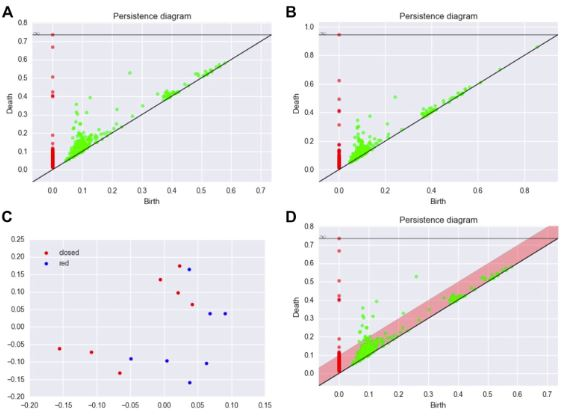
\includegraphics[width=0.85\linewidth]{./figures/Figura14.JPG}
    \caption{
        (A, B) Dos diagramas de persistencia para dos configuraciones de la MBP
        (Maltose-Binding Protein).
        (C) Configuraci\'on MDS (Multi-Dimensional Scaling)
        para la matriz de distancias de cuello de botella.
        (D) Diagrama de persistencia con regi\'on de confianza para la MBP.
    }
    \label{fig:Figura 14}
    \vspace{15pt}
\end{figure}

Se han propuesto una variedad de m\'etodos para estimar $\eta_{\alpha}$
en el estudio por Fasy et al. (2014)\cite{Fasy2014b}.
Estos m\'etodos recaen principalmente en los resultados de estabilidad
para diagramas de persistencia;
se pueden derivar conjuntos de confianza para diagramas
de los conjuntos de confianza en el espacio muestral.

\subsection*{Acercamiento por submuestreo}

Este m\'etodo se basa en una regi\'on de confianza para el soporte $K$
de la distribuci\'on de la muestra en la distancia de Hausdorff.
Sea $\tilde{\mathbb{X}_{b}}$ un submuestreo de tama\~{n}o $b$ de una muestra
$\tilde{\mathbb{X}_{n}}$, donde $b = o\cpar{n/\log n}$.
Sea $\mathrm{q}_{b}\cpar{1 - \alpha}$ un cuantil de la distribuci\'on de
$\mathrm{Haus}\cpar{\tilde{\mathbb{X}_{b}},\mathbb{X}_{n}}$.
Sea $\Hat{\eta}_{\alpha}:=2\Hat{q}_{b}\cpar{1-\alpha}$, donde
$\Hat{q}_{b}$ es una estimaci\'on $\mathrm{q}_{b}\cpar{1-\alpha}$ usando un
procedimiento de Monte Carlo est\'andar.
Bajo un supuesto $\cpar{a,b}$ est\'andar y para una $n$ suficientemente grande,
el estudio por Fasy et al. (2014)\cite{Fasy2014b} muestra que

\begin{equation*}
    P\cpar{
        \mathrm{d}_{b}\cpar{
            \mathrm{dgm}\cpar{\mathrm{Filt}\cpar{K}},
            \mathrm{dgm}\cpar{\mathrm{Filt}\cpar{\mathbb{X}_{n}}}
        }
        >\Hat{\eta}_{\alpha}
    }
    \leq
    P\cpar{
        \mathrm{Haus}\cpar{K,\mathbb{X}_{n}}>\Hat{\eta}_{\alpha}
    }
    \leq
\alpha+O\cpar{\frac{b}{n}}^\frac{1}{4}.
\end{equation*}

\section*{Bootstrap de Cuello de Botella}

Los resultados de estabilidad suelen llevar a conjuntos de confianza conservativos.
Una estrategia alternativa es el bootstrap de ceullo de botella
introducido en el estudio por Chazal et al. (2016)\cite{Chazal2016a}.
Consideramos el escenario general donde un diagrama de persistencia
$\Hat{\mathrm{dgm}}$ se define como la observaci\'on
$\cpar{X_{1},\dots,X_{n}}$ en un espacio m\'etrico.
Este diagrama de persistencia corresponde a la estimaci\'on de
un diagrama de persistencia subyacente $\mathrm{dgm}$,
que puede ser relacionado, por ejemplo, al soporte de la medida,
o al los conjutos subnivel de la funci\'on relacionada a esta distribuci\'on
(Por ejemplo, una funci\'on de densidad donde las $X_{i}$'s estan en
$\mathbb{R}^{d}$).
Sea $\cpar{X_{1}^{*},\dots,X_{n}^{*}}$ una muestra de una medida emp\'irica
definida de las observaciones $\cpar{X_{1},\dots,X_{n}}$.
Y sea $\widehat{\mathrm{dgm}}^{*}$ el diagrama de persistencia
derivado de esta muestra.
Podemos tomar entonces para $\eta_{\alpha}$ la cantidad $\Hat{\eta}_{\alpha}$
definida por:
\begin{equation}
    P\cpar{\mathrm{d_{b}}\cpar{
    \widehat{\mathrm{dgm}}^{*},\widehat{\mathrm{dgm}}}>\widehat{\eta}_{\alpha}|X_{1},\dots,X_{n}} 
    =\alpha.
\end{equation}
Es de notar que $\Hat{\eta}_{\alpha}$ puede ser estimada con facilidad utilizando
m\'etodos de Monte Carlo.
Se ha demostrado en el estudio por Chazal et al. (2016)\cite{Chazal2016b}
que el bootstrap de cuello de botella es una opci\'on v\'alida para calcular
los conjuntos subnivel de un estimador de densidad.

\section*{Bootstrap para N\'umeros de Betti Persistentes}

Como se ha mencionado, las regiones de confianza basadas en las propiedades de estabilidad
de la persistencia suelen dar lugar a regiones de confianza muy conservadoras.
Basados en los conceptos de estad\'isticos estabilizantes, Penrose y Yukick
(2001)\cite{PenroseYukich2001}, recientemente si ha mostrado normalidad asint\'otica para
n\'umeros de Betti persistentes en Krebs y Polonik (2019)\cite{KrebsPolonik2019},
y en Roycraft et al. (2020)\cite{Roycraft2020} bajo muy pocas condiciones en la filtraci\'on y
distribuci\'on de la nube muestral.
Adem\'as los procedimientos de bootstrapping tambi\'en son v\'alidos en este
acercamiento.
M\'as precisamente, un procedimiento bootstrap suavizado junto a un conveniente
reescalado de la nube de puntos, parece ser un acercamiento prometedor
para el bootstrapping de caracter\'isticas ATD de la nube de puntos de datos.

\section{Estad\'isticos para una Familia de Diagramas de Persistencia y Otras Representaciones}

Hasta ahora hemos considerado estad\'isticos basados solamente un diagrama de persistencia.
Dirigimos nuestra atenci\'on ahora a un nuevo esquema donde se encuentran a disposici\'on una
variedad de diagramas de persistencia (y otras representaciones),
y estamos interesados en proveer una tendencia central,
regiones de confianza y pruebas de hip\'otesis para descriptores topol\'ogicos
construidos en esta familia.

\subsection{Tendencia Central para la Homolog\'ia Persistente}

\textbf{\textit{\large Media de Distribuciones de Diagramas}}

Dado que el espacio de diagramas de persistencia es un espacio m\'etrico general pero no
un espacio de Hilbert, la definici\'on de media en diagramas de persistencia no es obvia ni
\'unica.
Un primer acercamiento natural para definir una medida de tendencia central en este contexto
es considerar la media de Fr\'echet de distribuciones de diagramas.
Su existencia ha sido demostrada en el estudio por Mileyko et al. (2011)\cite{Mileyko2011},
y tambi\'en han sido caracterizadas en el estudio por Turner er al. (2014)\cite{Turner2014a}.
Sin embargo, pueden no ser \'unicas, y resultan complicadas de calcular en la pr\'actica.
Algunos acercamientos para tratar de solucionar estas problematicas que se han propuesto
recientemente incluyen la propuesta basada en transporte \'optimo n\'umerico
Lacombe et al. (2018)\cite{Lacombe2018} as\'i como las representaciones lineales y m\'etodos
basados en el kernel por Divol y Chazal (2020)\cite{Divol2020}.\medbreak\medbreak

\textbf{\textit{\large Firmas Topol\'ogicas de Submuestras}}

Tambi\'en podemos usar propiedades de tendencia central de la homolog\'ia persistente para
calcular firmas topol\'ogicas para conjuntos de datos de gran tama\~{n}o,
como alternativa al prohibitivo costo de los c\'alculos de persistencia.
Dada una gran nube de puntos, la idea es extraer muchas submuestras,
calcular el paisaje de persistencia de cada submuestra, y luego combinar la informaci\'on.

Para cualquier entero positivo $m$, sea $X = \cllav{X_{1},\dots,x_{m}}$ un muestra de $m$ puntos
tomada de una medida $\mu$ en un espacio m\'etrico $M$
cuyo soporte es denotado por $\mathbb{X}_{\mu}$.
Suponemos que el diametro de $\mathbb{X}_{\mu}$ es finito
y acotado superiormente por $\frac{T}{2}$,
donde $T$ es la misma constante que en la definici\'on de paisajes de persistencia
en la Secci\'on \ref{sec: 4.4}.
Concentramos nuestra atenci\'on ahora en el caso de $k=1$ y el conjunto
$\lambda\cpar{t}=\lambda\cpar{1,t}$.
Sin embargo, los resultados que presentaremos a continuaci\'on se sostienen para $k>1$.
